\documentclass[12pt]{article}
\usepackage[utf8]{inputenc}
\usepackage{cite}
\usepackage[spanish]{babel}
\selectlanguage{spanish}
\usepackage{graphicx}
\graphicspath{ {files/} }
\usepackage{url}
\usepackage{natbib}




\title{Reporte sobre la Actividad 2}
\author{García Parra Pedro}
\date{Febrero 2019}

\begin{document}

\maketitle

En esta actividad aprendimos a utilizar la biblioteca pandas, la cual es una bliblioteca para python que te permite realizar un analisis sobre una serie de datos. También se utilizó la biblioteca matplotlib, más específicamente pyplot para ayudarnos en la graficación de algunos datos.

Para la realización de esta actividad se respondieron las siguientes preguntas:
\begin{itemize}
    \item ¿Cómo le podrás determinar cuáles son los meses más lluviosos?
    \item ¿Cuáles son los meses más fríos y cuáles son los más cálidos?
    \item ¿Cuáles han sido años muy húmedos? 
    \item ¿Cuáles han sido años muy secos?
    \item ¿Cuáles años han tenido inviernos fríos?
    \item ¿Cuáles años han tenido veranos más cálidos?
    \item ¿Cómo ha venido siendo la temperatura mensual promedio en los últimos 20 años? 
    \item ¿Qué ha pasado con la precipitación en los últimos 20 años de datos? 
\end{itemize}

Para responder las primeras cuatro preguntas usé la siguiente función de pandas:
\begin{verbatim}
    df.groupby(args)
\end{verbatim}
donde df es un objeto DataFrame y los argumentos que se le pasan es en base a qué se va a agrupar.

En particular para responder la primer pregunta se utilizó la siguiente única linea de código:
\begin{verbatim}
    df.groupby(df['FECHA'].dt.strftime('%B'))['PRECIP'].mean().sort_values()
\end{verbatim}
\begin{figure}
    \centering
    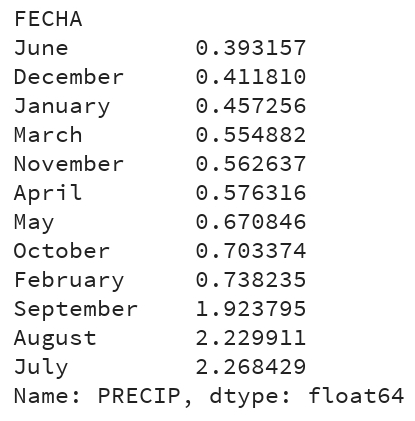
\includegraphics[scale = .5]{tabla.png}
    \caption{Output para la resolución de la primer pregunta}
    \label{fig:linea1}
\end{figure}
El resultado de ejecutar esa línea es la tabla que se muestra en la figura (\ref{fig:linea1}) y con ella podemos ver cual fue el mes en que hubo menos precipitacion y el cual hubo más.
Las tres preguntas siguientes son similares.

Para la pregunta cinco primero tuve que obtener la temperatura minima solamente de los meses de invierno (Diciembre, Enero, Febrero y Marzo) para eso primero obtuve los indices en mi dataFrame en los cuales era invirno, luego cree un array donde guardé las temperaturas de estos días y por ultimo utilizé df.groupby() para ordenarlos de acuerdo al año; el codigo que utilicé fue el siguiente:
\begin{verbatim}
## Obtiene el indice de los datos que se encuentran en invierno 
##(mes entre diciembre y marzo)
Invi = []
j = 0
for i in range(0,7790):
    if (df["MES"][i] == 12 or df["MES"][i] == 1 or df["MES"][i] == 2 
        or df["MES"][i] == 3):
        Invi.append(i)

## Crea el array con los años y temperaturas
años = []
temp = []
inv = []
for i in Invi:
    años.append(df["AÑO"][i])
for i in Invi:
    temp.append(df["TMIN"][i])
inv = [años,temp]
inviernos = pd.DataFrame({
    'AÑOS': inv[0],
    'TMIN': inv[1]},
    index = range(0,len(años)))
## Muestra los valores de la media de la temperatura
inviernos.groupby("AÑOS")['TMIN'].mean().sort_values()
\end{verbatim}

El resultado de ejecutar este codigo es similar a la figura(\ref{fig:linea1}) y se puede responder la pregunta de manera muy sencilla.
La pregunta seis fue realizada de la misma manera.

Para realizar las preguntas 7 y 8 cree un dataFrame nuevo donde se omitieran los datos de 1990 y 1991 para así tener solamente los ultimos 20.
Tras realizar eso solamente se volvio a utilizar la función groupby() y encontrar la respuesta de la pregunta fue muy sencillo.


\end{document}
